\section{Criteria Limitations for GFM converters}
\label{sec:lim}

In this section, we illustrate why the stability conditions of Theorem \ref{thm:dec_mixed_small_gain_phase} are difficult to be satisfied in practical power system applications.
A typical example arises with grid-forming (GFM) converters, which often exhibit high low-frequency gain.
%Under such conditions, the small-gain condition is not satisfied. At the same time, the converter impedance matrix may fail to be sectorial at those same frequencies, rendering the small-phase condition inapplicable.
To demonstrate this limitation, we consider a conventional GFM converter implementing virtual synchronous machine (VSM) power control (described in detail in Appendix \ref{apx:GFM_control}) connected to an infinite bus, see Figure \ref{fig:gfm_diag}, through a network with low short-circuit ratio (SCR), i.e., large grid impedance. The resulting small-gain and small-phase plots for the feedback loop are shown in Figure~\ref{fig:GFM_gain_phase_test}.

Three main issues arise from this example:
\begin{itemize}
    \item Violation of the small-gain condition: the gain of the converter significantly exceeds that of the grid. As a result, the small-gain condition is never satisfied.
    \item Violation of sectoriality: below $0.9$ Hz, the converter impedance is not sectorial, and therefore the small-phase criterion cannot be applied. 
    \item Conservativeness: even when the admittance is sectorial and the phase is well-defined, the phase intervals of the converter and the grid are very close to overlapping for frequencies below $50$ Hz, and eventually do overlap near $1$ Hz. This overlap is not necessarily indicative of an actual instability but is instead a consequence of the conservativeness of the small-phase criterion.
\end{itemize}
%Although the latter issue is less restrictive than the first two, it nonetheless represents a practical limitation that can hinder the applicability of the method. Later in the paper, we revisit this problem and propose a solution to mitigate such conservativeness.
From this example, it is clear that the classical small-gain and small-phase criteria exhibit significant limitations in realistic converter-dominated scenarios. A detailed examination is now presented in the following subsection to identify the source of this non-sectoriality.
\begin{figure}[tbh]
    \centering
    \begin{subfigure}{\columnwidth}
        \centering
        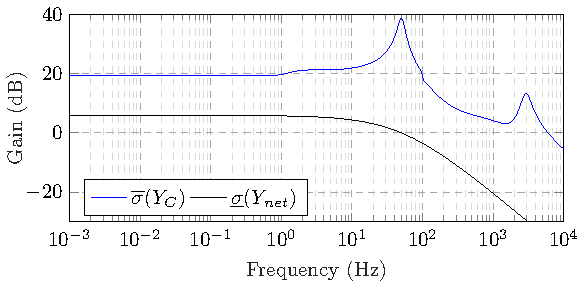
\includegraphics[width=\linewidth]{Gain_adm.pdf}
    \end{subfigure}
    \begin{subfigure}{\columnwidth}
        \centering
        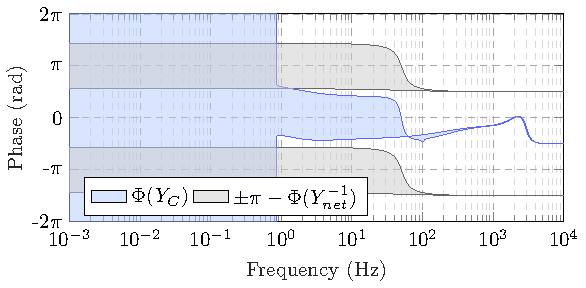
\includegraphics[width=\linewidth]{Phase_adm.pdf}
    \end{subfigure}
    \caption{Mixed small gain–phase condition for a GFM converter. If a system is not sectorial, its phase is represented by the full interval $[-2\pi,\, 2\pi]$. The small-gain condition is violated if the converter gain exceeds the network gain. The small-phase condition is violated if the converter phase overlap the network phase shifted by $\pm\pi$.}
    \label{fig:GFM_gain_phase_test}
\end{figure}

\subsection{Non-Sectoriality of GFM converter}
As illustrated in the previous example, and also reported in other studies, converter admittances are often non-sectorial at low frequencies \cite{huangGainPhaseDecentralized2024,woolcockMixedGainPhase2023}. However, the origin of this phenomenon has not been thoroughly investigated, and it remains unclear whether it is a consequence of specific control architectures and parameter choices, or an intrinsic property of the device itself.

We adopt the modeling approach described in \cite{guImpedanceBasedWholeSystemModeling2021}. The small-signal admittance model of a generic converter is depicted in Figure~\ref{fig:frame_embedding}. The input to the model is the voltage at the point of common coupling, $V_{DQ}$, expressed in a local steady $DQ$ reference frame, while the output is the converter current $I_{DQ}$ in the same frame. The converter controller operates in a local swing $dq$ reference frame, and is conceptually divided into two parts: 
\begin{itemize}
    \item Synchronization controller $K_v(s)$, which generates the angle $\epsilon$ used to transform variables from the local steady to the swing frame.
    \item Remainder of the control system $Y_{dq}(s)$, which includes the current control, voltage control, virtual impedance, reactive power control, and other controllers not related to the synchronization.
\end{itemize}
 The closed-loop admittance in the local steady frame can then be written as~\eqref{eq:frame_embedding}. The vectors $V_0^e=[-V_{q,0},V_{d,0}]^T$ and $I_0^e=[-I_{q,0},I_{d,0}]^T$ represent the linearized rotation terms between the two frames, where $V_{d,0}$, $V_{q,0}$, and $I_{d,0}$, $I_{q,0}$ are the voltage and current operating points.
\begin{equation}
    Y_{DQ}(s)=(Y_{dq}(s)+I_0^eK_v(s))(I+V_0^eK_v(s))^{{-}1}
    \label{eq:frame_embedding}
\end{equation}
 \begin{figure}
     \centering
     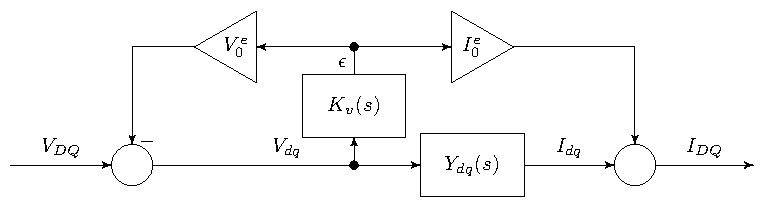
\includegraphics[width=\linewidth]{frame_embedding.pdf}
     \caption{Small-signal model of a generic converter with synchronization frame embedding.}
     \label{fig:frame_embedding}
 \end{figure}
For a typical GFM converter with power synchronization, the angle $\epsilon$ is generated by a dynamic system of the form~\eqref{eq:freq_tf}, where $\omega$ denotes the frequency, $P$ is the active power, and $H_P(s)$ is the transfer function of the power-based synchronization loop. 
\begin{equation}
    \omega = H_P(s)P\,,\quad \epsilon=\frac{1}{s}\omega
    \label{eq:freq_tf}
\end{equation}
Linearization of the power expression yields \eqref{eq:power_lin}, in which $P$ depends only on the voltage in the local steady frame, allowing $K_v(s)$ to be written as~\eqref{eq:Kv}.
\begin{equation}
    P \approx \underbrace{(V_0 Y_{dq}+I_o)}_{:=G_P(s)} V_{dq}\,,\, V_0=[V_{d,0} \, V_{q,0}], \, I_0=[I_{d,0} \, I_{q,0}]
    \label{eq:power_lin}
\end{equation}
\begin{equation}
    K_v(s) = \frac{H_P(s)}{s}G_P(s)
    \label{eq:Kv}
\end{equation}
Since our focus is on the low-frequency behavior, we consider the DC gain of the admittance at $s=j0$. The following proposition summarizes the key result.
\begin{prop}
    Assume $V_{q,0}=0$, $V_{d,0}\neq0$, and $K_v(s)V_0^e$ is not identically zero. The converter admittance matrix \eqref{eq:frame_embedding} with $K_v(s)$ as in \eqref{eq:Kv} evaluated at $s=0$ is equal to:
\begin{equation}
    Y_{DQ}(0)=\begin{bmatrix}
        -\frac{I_{d,0}}{V_{d,0}} & -\frac{I_{q,0}}{V_{d,0}} \\
        \beta & \frac{I_{d,0}}{V_{d,0}}
    \end{bmatrix}
    \label{eq:Y_DQ_0}
\end{equation}
for some $\beta$. Moreover, $Y_{DQ}(0)$ is not sectorial.
\label{prop:Y_DQ_0}
\end{prop}
\begin{proof}
    The derivation of \eqref{eq:Y_DQ_0} is given in Appendix \ref{apx:Prop_Y_DQ_0}. 
    Since the trace is null, then the eigenvalues' sum is zero. The numerical range of a $2\times2$ matrix is an ellipse with the two eigenvalues as foci. Depending on the values of $\beta$ and $I_{q,0}$, the ellipse has as principal axis either the real axis or the imaginary axis. In both cases, the origin belongs to the numerical range, making the matrix not sectorial.
\end{proof}

The assumption $V_{q,0}=0$ is without loss of generality since a rotation matrix can always be chosen so that this holds. Furthermore, depending on the converter operating point and the parameters, not only the admittance is non-sectorial but also non-quasi-sectorial.
This result demonstrates that, regardless of the control implementation, sectoriality cannot be achieved at 0 Hz and will generally not be satisfied at low frequencies. The root cause lies in the fact that a GFM converter behaves as a constant power load/source. Even when frequency droop is implemented (so that power varies with frequency), from the admittance perspective (voltage-to-current relation) the converter still behaves as a constant power device.
Furthermore, the above analysis shows that the converter is not passive\footnote{Here, “passive” is used in the loose frequency-wise sense common in the power electronics literature, referring to positive realness of $Y(j\omega)$.} at low frequency. This finding is consistent with previous work \cite{deyAnalysisPassivityCharacteristics2021}, but is more general in scope as it does not depend on a specific control implementation or parameter values.

\begin{rem}
    A similar analysis can be carried out for grid-following (GFL) converters. For instance, with an SRF-PLL synchronization loop, 
    $K_v(s)$ takes the form $\frac{H_{PLL}(s)}{s}[0,1]$.
    %$G_P(s)$ is replaced with the vector $[0,1]$. 
    For a typical PI-based active power control, the resulting admittance has the same form as in \eqref{eq:Y_DQ_0}. 
    Therefore, the same considerations regarding low-frequency non-sectoriality and lack of passivity apply to GFL converters as well.
\end{rem}